% EHB415 PRS yerlesimi gorsel karti. Derleme (ogretici klasorunde): C:\Users\Huawei\tools\tectonic\tectonic.exe -X compile gorev_karti_prs_gorsel.tex
\documentclass[11pt,a4paper]{article}
\usepackage{fontspec}
\setmainfont{georgia}[Path=./fontlar/,Extension=.ttf,BoldFont=georgiab,ItalicFont=georgiai,BoldItalicFont=georgiaz]
\setsansfont{arial}[Path=./fontlar/,Extension=.ttf,BoldFont=arialbd,ItalicFont=ariali,BoldItalicFont=arialbi]
\setmonofont{consola}[Path=./fontlar/,Extension=.ttf,BoldFont=consolab,ItalicFont=consolai,BoldItalicFont=consolaz,Scale=0.88]
\usepackage[a4paper,left=2cm,right=2cm,top=1.8cm,bottom=1.8cm]{geometry}
\usepackage{xcolor,booktabs,enumitem,graphicx}
\usepackage[most]{tcolorbox}
\usepackage{fancyhdr,titlesec}
\definecolor{ink}{HTML}{1F2937}\definecolor{acc}{HTML}{1D4ED8}\definecolor{accl}{HTML}{DBEAFE}
\definecolor{warn}{HTML}{EA580C}\definecolor{warnl}{HTML}{FFEDD5}\definecolor{muted}{HTML}{6B7280}
\color{ink}
\titleformat{\section}{\sffamily\bfseries\Large\color{acc}}{}{0pt}{}[{\color{acc!35}\titlerule[1pt]}]
\titleformat{\subsection}{\sffamily\bfseries\normalsize\color{acc!80!black}}{}{0pt}{}
\titlespacing*{\section}{0pt}{4pt}{8pt}\titlespacing*{\subsection}{0pt}{8pt}{3pt}
\setlength{\parindent}{0pt}\setlength{\parskip}{5pt}
\setlist{itemsep=4pt,topsep=3pt,parsep=0pt}
\pagestyle{fancy}\fancyhf{}\renewcommand{\headrulewidth}{0.3pt}
\fancyhead[L]{\sffamily\footnotesize\color{muted} EHB415 \textbullet\ PRS yerleşimi (görsel kart)}
\fancyfoot[C]{\sffamily\footnotesize\color{muted}\thepage}
\newtcolorbox{amac}{enhanced,colback=accl,colframe=acc,boxrule=0.5pt,arc=2pt,left=6pt,right=6pt,top=4pt,bottom=4pt,
  fonttitle=\sffamily\bfseries\small,title=Amaç,coltitle=white,colbacktitle=acc,
  attach boxed title to top left={yshift=-2mm,xshift=4mm},boxed title style={arc=2pt,boxrule=0pt}}
\begin{document}

\section*{PRS yerleşimi: ızgarada PRS nerede duruyor?}
{\sffamily\color{muted} Bu kart tablo değil, resim. Her resmin altında ne gördüğünü ve nereden bildiğimizi yazdım. Yanında \texttt{ogretici/veri/prs\_gorsel.xlsx} var: oradan bir PRS ayarı seçince aynı resimler değişiyor.}

\begin{amac}
PRS'in ızgarada üç yerde yer tuttuğunu görmek: bir PRB'nin \emph{içinde} (hangi kutular), \emph{zamanda} (hangi slotlar) ve \emph{frekansta} (hangi PRB'ler). Sonra bunun neden veriyi kapattığını görmek.
\end{amac}

\subsection*{Ayarlar ne demek}
\begingroup\sffamily\small
\begin{tabular}{@{}p{3.0cm}p{13.0cm}@{}}
\toprule
\textbf{Kutu} & Izgarada 1 alt taşıyıcı $\times$ 1 sembol. (Daha önce kutu = 1 PRB $\times$ 1 sembol demiştik; burada bir PRB'nin içine bakıyoruz, o yüzden kutu daha küçük.) \\
\textbf{periyot} & PRS kaç slotta bir geliyor. 30 kHz'te 1 slot = 0,5 ms. \\
\textbf{sembol} & Her PRS gönderimi kaç sembol sürüyor. \\
\textbf{comb} & PRS her kaç alt taşıyıcıdan birini dolduruyor. Comb 4: dörtte bir. \\
\textbf{bw} & PRS kaç PRB geniş. \\
\textbf{sembol ofseti} & PRS slotun kaçıncı sembolünden başlıyor. \\
\textbf{CORESET0} & PDCCH'nin (``kim veri alacak'' mesajı) durduğu yer. Bizde sembol 0, 48 PRB geniş (ön gözlem). \\
\textbf{veri alanı} & Verinin (PDSCH) kullanabildiği PRB'ler. Ölçümümüzde ilk 48 PRB. \\
\bottomrule
\end{tabular}
\endgroup

\subsection*{1. Bir PRB'nin içi}
\begin{center}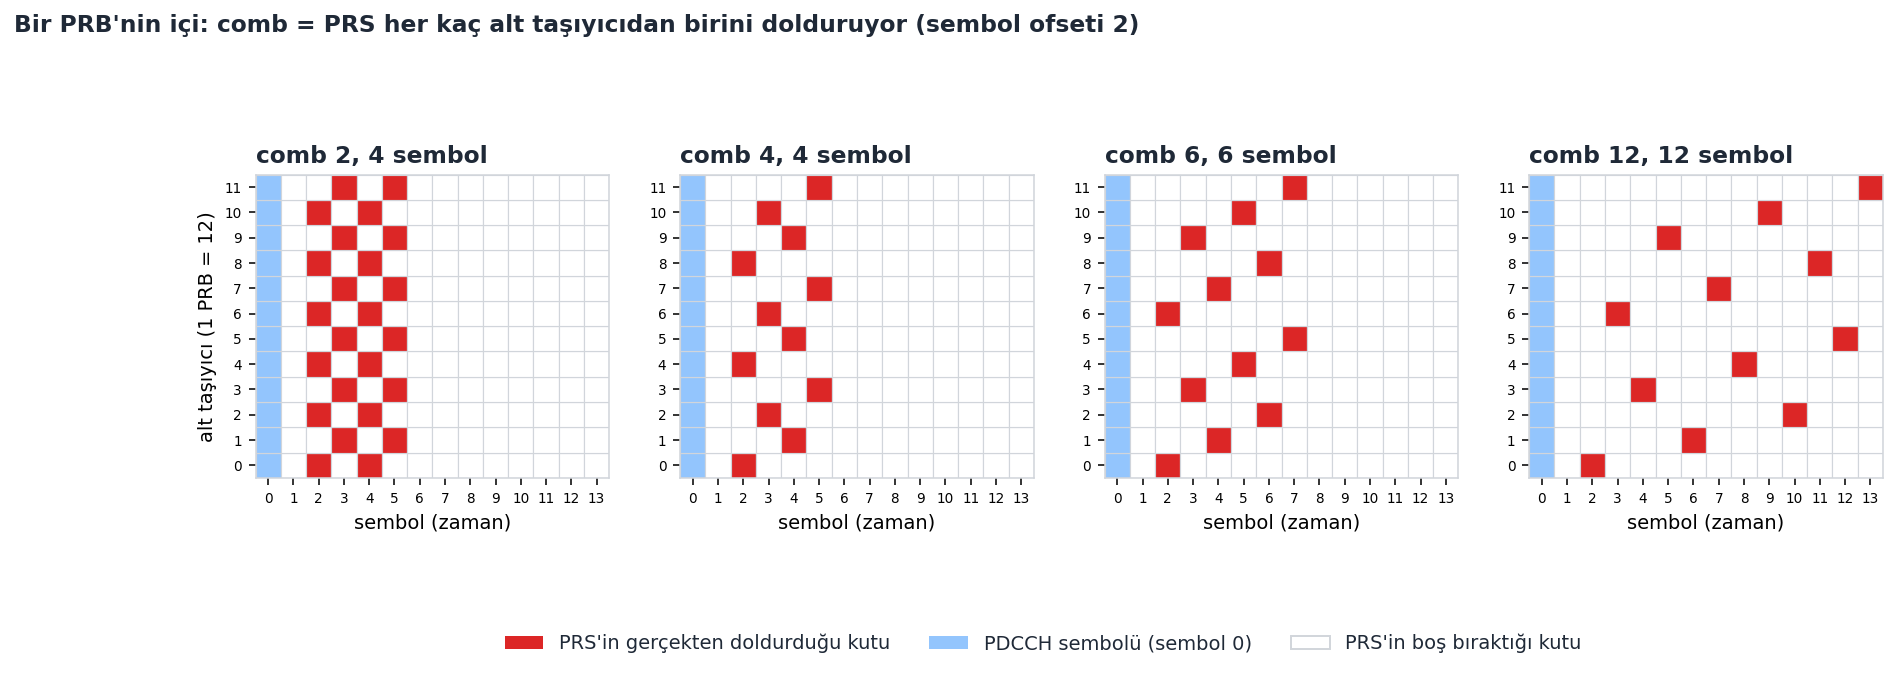
\includegraphics[width=\textwidth]{sekiller/prs_re_comb.png}\end{center}
Her ızgara 1 PRB: 12 alt taşıyıcı (dikey) $\times$ 14 sembol (yatay). Kırmızı kutular PRS'in gerçekten doldurduğu kutular. Comb büyüdükçe PRS daha seyrek, ve her sembolde başka bir alt taşıyıcıya kayarak ilerliyor; PRS bu yüzden ``merdiven'' çiziyor. \textbf{Kaynak:} desen OCUDU kodundan (\texttt{lib/ran/prs/prs.cpp}, \texttt{get\_prs\_freq\_offset}); comb 4 için sıra 0, 2, 1, 3.

\clearpage
\subsection*{2. Zamanda}
\begin{center}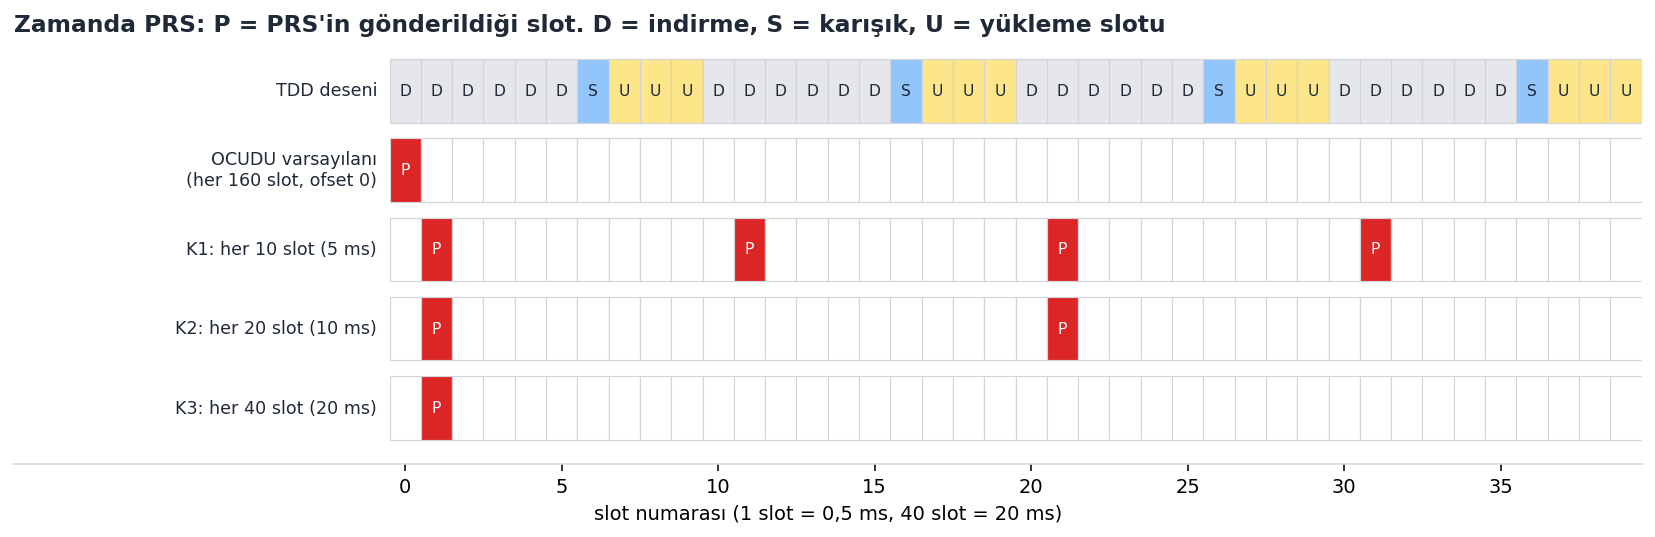
\includegraphics[width=\textwidth]{sekiller/prs_zaman.png}\end{center}
Üst satır TDD deseni: 6 indirme (D), 1 karışık (S), 3 yükleme (U) slotu, her 10 slotta tekrar. \textbf{OCUDU varsayılanı} PRS'i 160 slotta bir gönderir (80 ms), yani bu 40 slotluk pencerede yalnız ilk slotta görünür. K1, K2, K3 periyodu 10, 20, 40 slot yapar (5, 10, 20 ms). PRS indirme (D) slotlarına düşüyor. \textbf{Kaynak:} varsayılan değerler \texttt{du\_high\_config.h}; TDD deseni OCUDU varsayılanı; K1--K3 ortak dosyadaki öneri.

\subsection*{3. Frekansta}
\begin{center}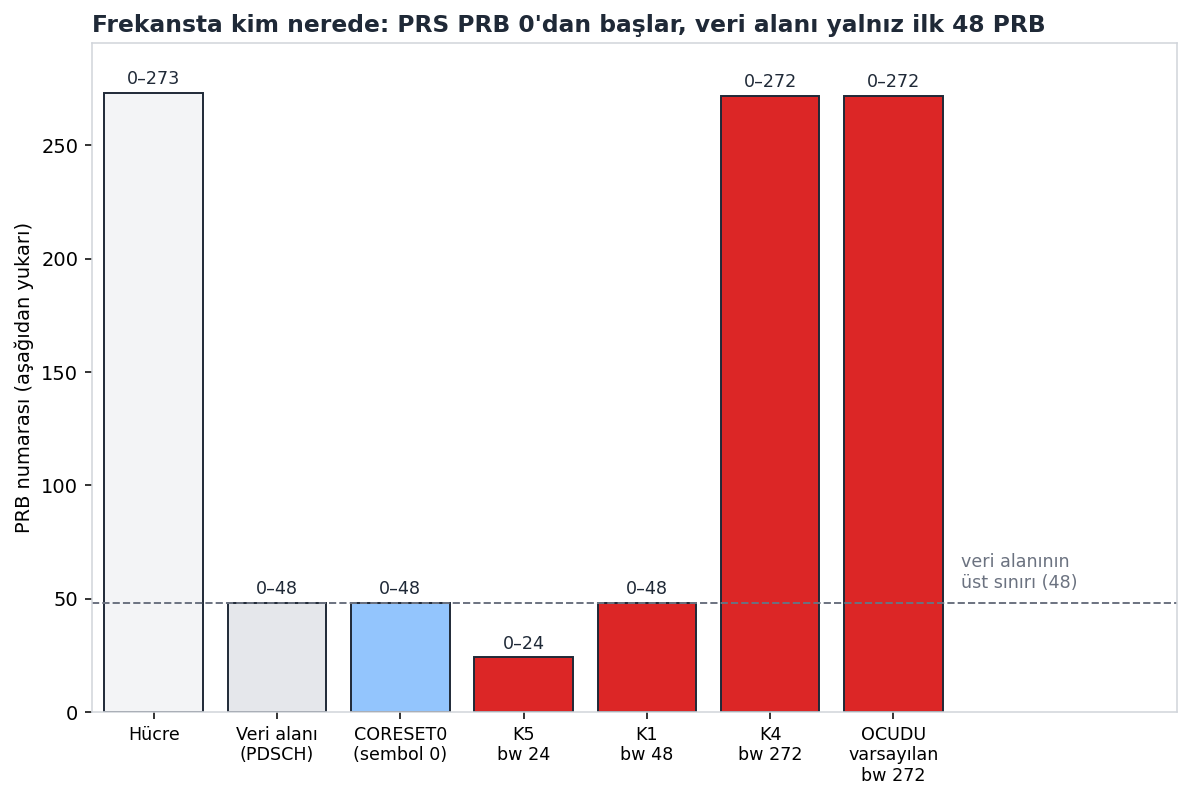
\includegraphics[width=0.78\textwidth]{sekiller/prs_frekans.png}\end{center}
PRS PRB 0'dan başlıyor (ayar verilmeyince varsayılan 0). Veri alanı (PDSCH) ve CORESET0 ilk 48 PRB. PRS 24 PRB ise veri alanının yarısını, 48 PRB ise tamamını, 272 PRB ise tamamını ve fazlasını kaplıyor. \textbf{Kaynak:} PDSCH aralığı \texttt{ocudu\_veri\_genislik.sh} çıktısı, \texttt{rb=[0..48)} (ölçüm, tek koşu); CORESET0 genişliğinin 48 olması ön gözlem.

\clearpage
\subsection*{4. Bir PRS slotunun içi: neden veri kapanıyor?}
\begin{center}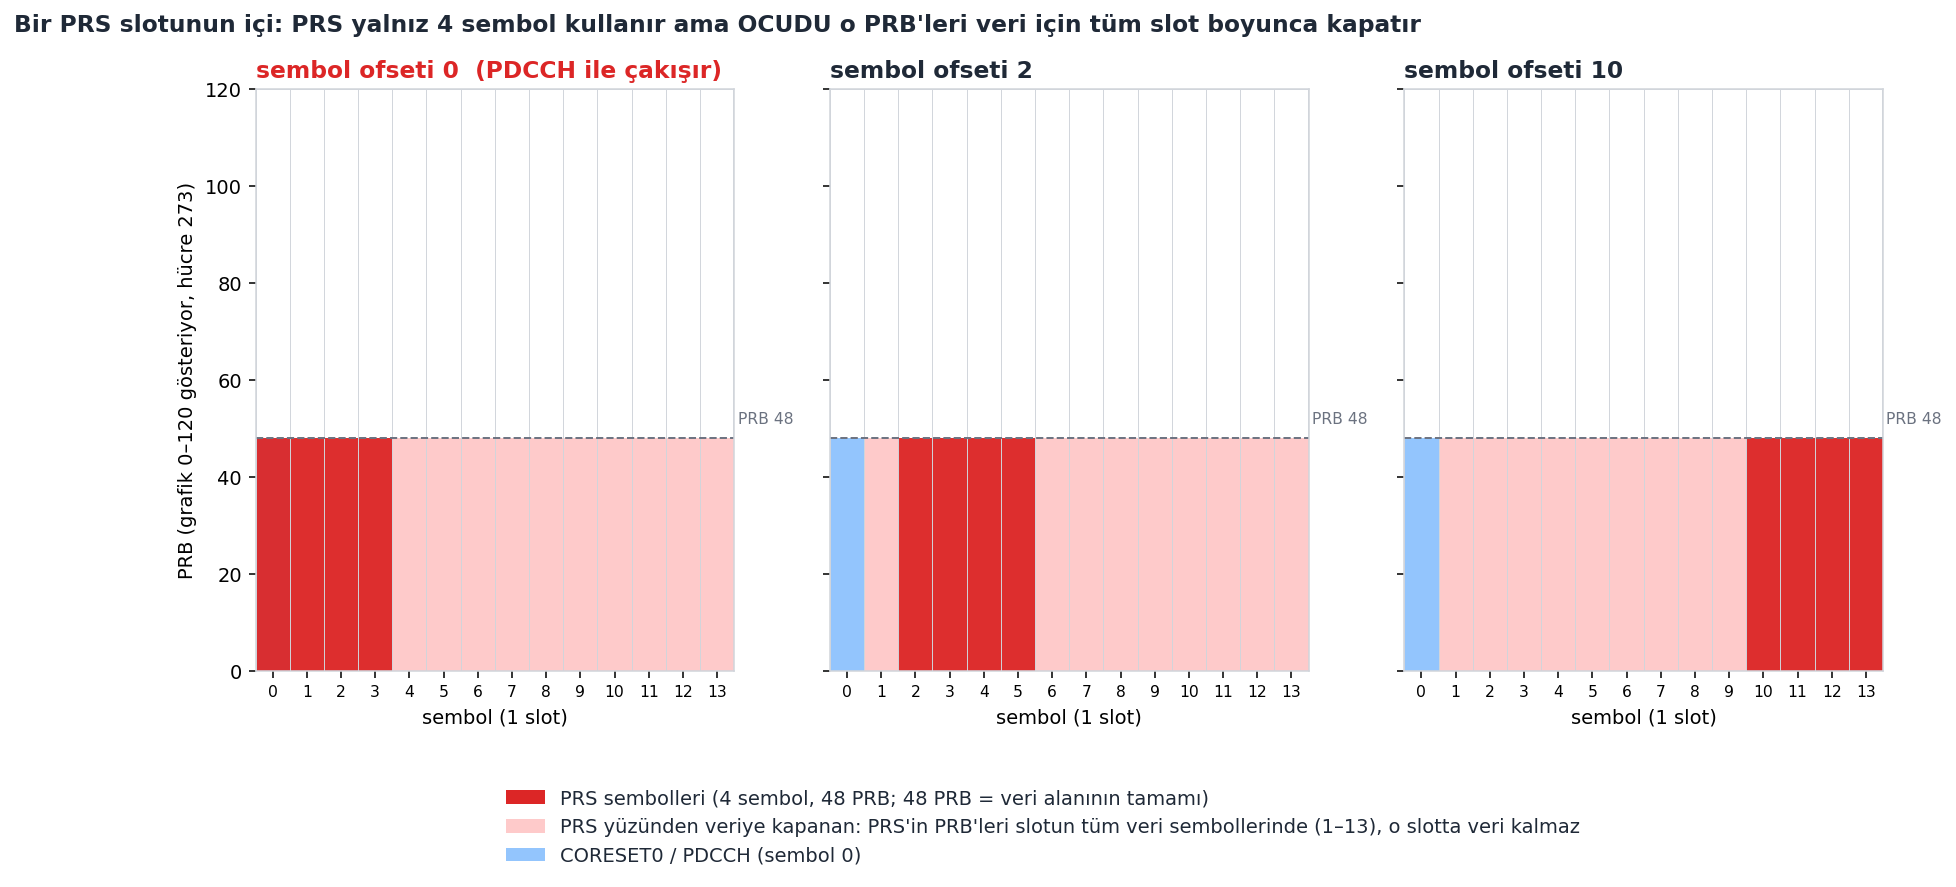
\includegraphics[width=\textwidth]{sekiller/prs_slot_ici.png}\end{center}
Koyu kırmızı: PRS'in sembolleri (burada 4 sembol). Açık kırmızı: PRS'in kullanmadığı ama veriye kapanan kutular. OCUDU, PRS'in PRB'lerini verinin kullanabileceği bütün sembollerde (1--13) dolu sayıyor. Kanıt iki yerde: (1) ölçüm: PRS 4 sembol de olsa 12 sembol de olsa DL aynı çıktı (\texttt{ocudu\_prs\_sweep.csv}, p4 ve p4s4: 43,8 Mbps); (2) kod: \texttt{intra\_slice\_scheduler.cpp} satır 874--896 (Fatih'in raporu, ben de kodu okudum). Ofset 0'da PRS sembol 0'a da giriyor ve PDCCH ile çakışıyor; eski testte bu UL'yi düşürdü (Fatih'in ölçümü).

\subsection*{5. PRS'in boş bıraktığı kutular da haberleşmeye verilirse}
\begin{center}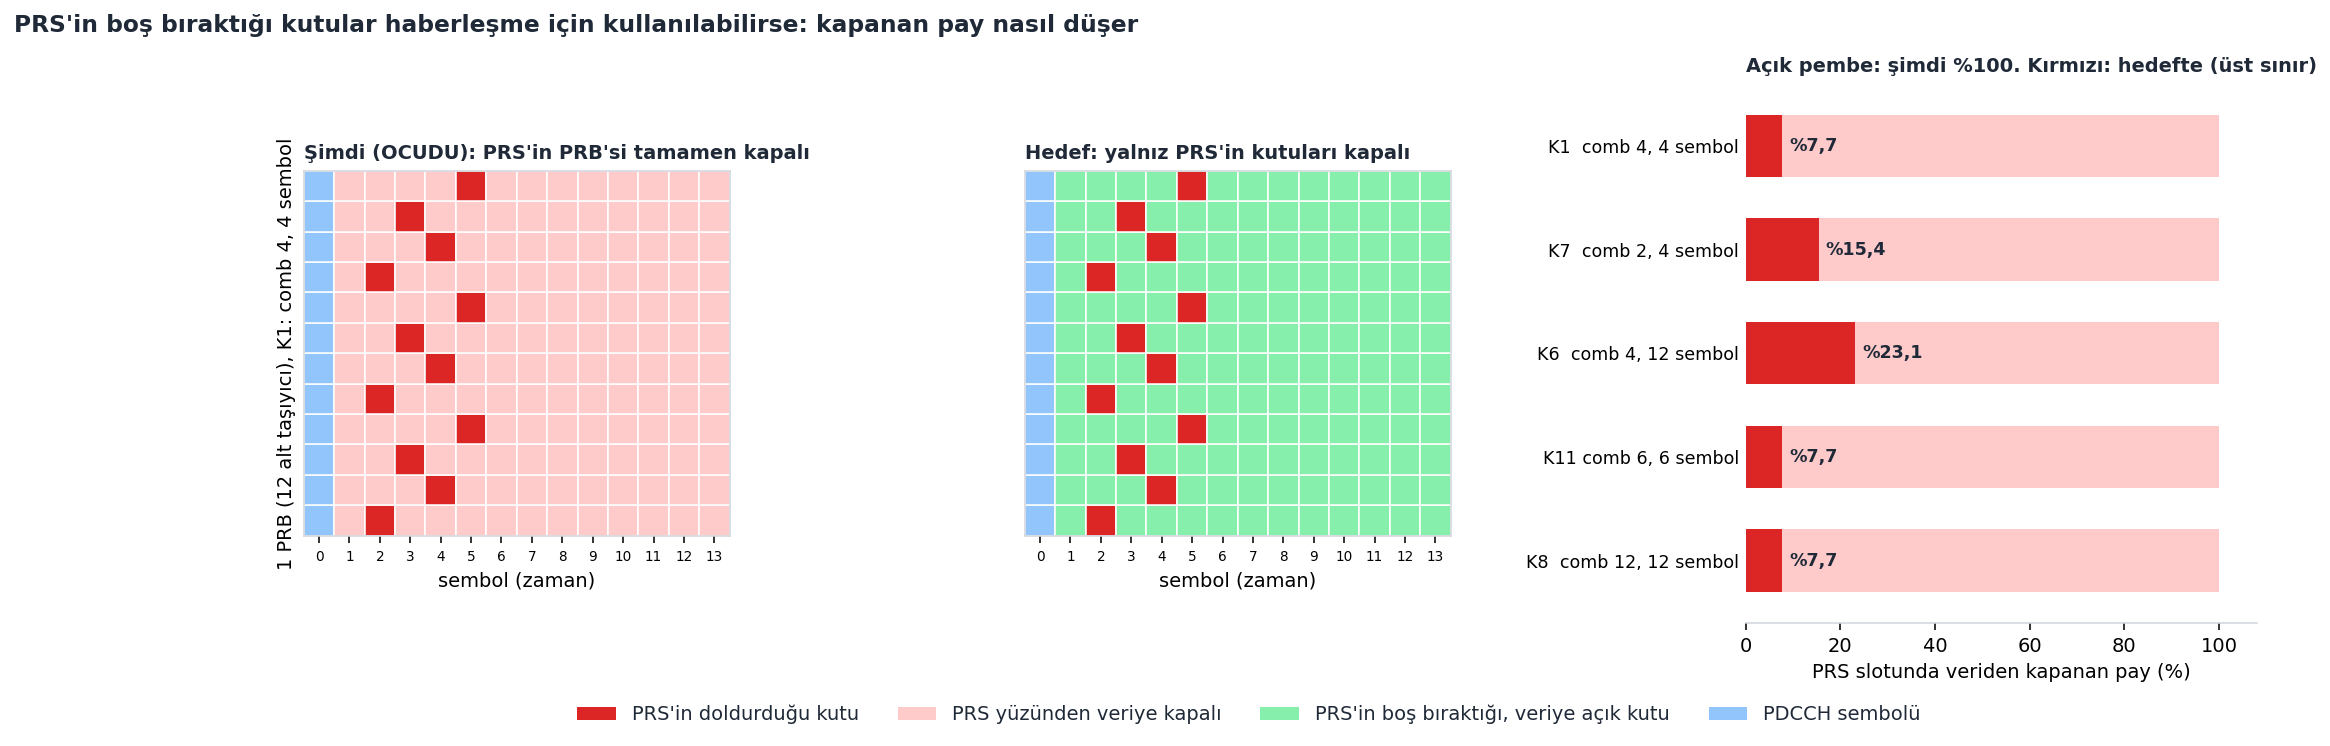
\includegraphics[width=\textwidth]{sekiller/prs_re_acik.png}\end{center}
OCUDU PRS'in bütün PRB'sini kapatıyor; kodda yorumu şöyle: \emph{``The resource grid is RB-granular, so the whole PRS bandwidth is reserved even though the resource only uses one subcarrier out of every comb size. There is no PDSCH rate matching around DL-PRS.''} (\texttt{prs\_scheduler.cpp} satır 189--192, okundu). Yani comb 6 ya da 12 seçmenin veriye hiçbir faydası yok: kapanan PRB aynı. Boş kutular veriye açılırsa PRS slotunda kapanan pay, PRS'in doldurduğu kutuların payına düşer: sembol sayısı $/ (13 \times \text{comb})$ (sağdaki grafik). \textbf{Bu bir hesap (üst sınır):} DMRS gibi başka ek yükleri saymadım, ve gerçek bir UE'nin bu kutuları nasıl atlayacağı (rate matching) açık soru.

\clearpage
\subsection*{Kendin dene (Excel, ``Seçici'' sayfası)}
\begin{enumerate}[leftmargin=1.6em]
\item B2'den K1'i, sonra K2'yi, sonra K3'ü seç. Slot çizelgesinde kırmızı sütunlar nasıl değişiyor? ``Veriden kapanan pay'' kaç çıkıyor? (Bizde: \%16,7, \%8,3, \%4,2.)
\item K4'ü seç. K1 ile karşılaştır: kapanan pay neden aynı çıkıyor, ama kırmızı alan neden daha uzun?
\item K9'u seç. Hangi hücre uyarı veriyor ve neden?
\item ``OCUDU varsayılan''ı seç. Slot çizelgesinde ne görüyorsun, kapanan pay kaç?
\item K6, K8 ve K11'i seç. ``PRS slotunda kapanan: RE düzeyi'' kaç çıkıyor? Comb büyüyünce neden düşüyor?
\end{enumerate}
{\sffamily\small\color{muted} Kontrol: K4'te pay K1 ile aynı (\%16,7), çünkü veri alanı yalnız 48 PRB. K9'da PDCCH çakışması ``VAR'' olur. OCUDU varsayılanında yaklaşık \%1,0. RE düzeyi: K6 \%23,1, K8 \%7,7, K11 \%7,7. Bu paylar bir \emph{modeldir}; TDD için ölçümle doğrulanmadı.}

\end{document}
